\newcommand{\teta}{\tilde{\eta}}

Incompressible flow represents the zero-Mach number limit of fluid
flow---no compressibility effects are modeled.  We can extend the
ideas of incompressibe flow to allow us to model some compressibility
effects, giving rise to low Mach number methods.

\section{Low Mach divergence constraints}

The key idea in solvers for low Mach number flows is that, as a fluid
element advects, its pressure remains the same as the background
state.  For an atmosphere, this background state is a hydrostatic
profile.  For a smallscale combustion flow, this background state is a
spatially constant pressure (and constant-in-time if the domain is
open).  We'll denote this background pressure as $p_0(r,t)$, where 
$r$ is a radial coordinate.

From the first law of thermodynamics, $Tds = de + pd(1/\rho)$, we see
\begin{equation}
T \frac{Ds}{Dt} = \frac{De}{Dt} + p_0 \frac{D(1/\rho)}{Dt}
\end{equation}
which is our internal energy evolution equation.  The internal
energy in a fluid parcel can change due to local heat release and 
diffusion, so we can write:
\begin{equation}
T \frac{Ds}{Dt} = \frac{De}{Dt} + p_0 \frac{D(1/\rho)}{Dt} = H +
\nabla \cdot (k \nabla T) \equiv \dot{q}
\end{equation}
where $H$ is the specific energy generation rate (energy / mass /time)
and $k$ is the thermal conductivity.

We can derive the constraint on the velocity field by considering the
Lagrangian derivative of the pressure---this captures the change in
pressure of a fluid element as it moves through the domain.
\begin{equation}
\frac{Dp_0}{Dt} = \left . \frac{\partial p_0}{\partial \rho} \right |_s
     \frac{D\rho}{Dt} +
     \left . \frac{\partial p_0}{\partial s} \right |_\rho
     \frac{Ds}{Dt}
\end{equation}
we recognize that $\Gamma_1 \equiv \partial \log p_0/\partial \log \rho |_s$.
The Maxwell relations tell us that
\begin{equation}
\partial p_0/\partial s |_\rho = \rho^2 \partial T/\partial \rho |_s
\end{equation}
This gives us the form:
\begin{equation}
\frac{Dp_0}{Dt} = \frac{p_0}{\rho} \Gamma_1 \frac{D\rho}{Dt} +
     \left . \rho^2 \frac{\partial T}{\partial \rho} \right |_s
     \frac{\dot{q}}{T}
\end{equation}

We need an expression for $\partial T/\partial \rho |_s$ and terms of
derivatives of $\rho$ and $T$ (since that is what our equations of
state typically provide).  Consider $\Gamma_1$, with $p = p(\rho, T)$:
\begin{equation}
  \Gamma_1 = \frac{\rho}{p} \left . \frac{dp}{d\rho} \right |_s
  = \frac{\rho}{p} \left [ p_\rho + p_T \left . \frac{dT}{d\rho} \right |_s \right ]
\end{equation}
where we use the shorthand $p_\rho \equiv \partial p/\partial \rho |_T$ and
$p_T \equiv \partial p/\partial T |_\rho$.  This tells us that
\begin{equation}
  \left . \frac{\partial T}{\partial \rho} \right |_s = \frac{p}{\rho p_T} (\Gamma_1 - \chi_\rho)
\end{equation}
where $\chi_\rho \equiv \partial \log p / \partial \log \rho |_T$.  Using the following
relations
\begin{equation}
\frac{\Gamma_1}{\chi_\rho} = \frac{c_p}{c_v}
\end{equation}
and
\begin{equation}
  c_p - c_v = \frac{p}{\rho T} \frac{\chi_T^2}{\chi_\rho}
\end{equation}
with $\chi_T \equiv \partial \log p / \partial \log T |_\rho$
(see, e.g. \cite{HKT} for both of these relations), we can
write
\begin{equation}
  \left . \frac{\partial T}{\partial \rho} \right |_s = \frac{p\chi_T}{\rho^2 c_v}
\end{equation}

Putting this all together, we have:
\begin{equation}
\frac{Dp_0}{Dt} = \frac{p_0}{\rho}\Gamma_1  \frac{D\rho}{Dt}
   + \frac{p \chi_T}{c_v T} \dot{q}
\end{equation}
The continuity equation gives us:
\begin{equation}
\frac{D\rho}{Dt} = -\rho \nabla \cdot U
\end{equation}
Solving for the velocity divergence, 
we finally have:
\begin{align}
  \nabla \cdot U + \frac{1}{\Gamma_1 p_0}\frac{Dp_0}{Dt} &=
    \frac{\chi_T }{c_v T \Gamma_1} \dot{q} 
  = \frac{\chi_T}{c_p \chi_\rho T} \dot{q} \nonumber \\
 &= \frac{p_T}{\rho c_p p_\rho} \dot{q}
  \equiv \sigma \dot{q}    
\end{align}
with
\begin{equation}
\sigma = \frac{\partial p_0/\partial T |_\rho}{\rho c_p \partial p_0/\partial \rho |_T}
\end{equation}
The $\sigma$ notation follows from \cite{ABRZ:II}, where we abbreviate
the righthand side as $S$.

This is the general constraint equation for low Mach flow.  Note that the
only approximation we made is $p \rightarrow p_0$.  This form of the constraint,
for a general equation of state, was originally derived in \cite{ABRZ:I}.  

\subsubsection{Combustion limit}

A useful limit is smallscale combustion.  In an open domain, we can take
$p_0$ as constant, so $Dp_0/Dt = 0$, and we are left with
\begin{equation}
\nabla \cdot U = S
\end{equation}
This looks like the constraint for incompressible flow, but with a source
to the divergence.  This source captures the compressible effects due
to local heat release---as a fluid parcel moves, the only changes to
its density will come through local heat release.  Methods for this
type of constraint are discussed in \cite{pember-flame,DayBell:2000,SNpaper}.

\subsubsection{Atmospheric case}

Another interesting case is that of an atmosphere.  If we consider an
ideal gas, then $\Gamma_1 = \gamma = \mathrm{constant}$.  A second
appromation we take is that $p_0 = p_0(r)$---i.e., no time
dependence to the atmosphere.  Finally, we'll consider the case
with no local heat sources ($S = 0$).  Then we have
\begin{equation}
\nabla \cdot U + \frac{1}{\gamma p_0} U \cdot \nabla p_0 = 0
\end{equation}
which is equivalent to
\begin{equation}
\nabla \cdot \left ( p_0^{1/\gamma} U \right ) = 0
\end{equation}
This constraint captures the changes in compressibilty due to the 
background stratification of an atmosphere.  This form was originally
derived for atmospheric flows by \cite{durran:1989} and generalized to
stellar flows in \cite{ABRZ:I}.  If the structure of the
atmosphere is isentropic, then we know that $d\log p_0 = \gamma d\log \rho_0$,
where we use $\rho_0$ to represent the density corresponding to $p_0$, and
we can write this constraint as:
\begin{equation}
\nabla \cdot (\rho_0 U) = 0
\end{equation}
This is the traditional anelastic constraint.

Extensions involving external heating sources or reactions are
discussed in \cite{ABRZ:II,ABNZ:III}, and dealing with the
non-constant $\Gamma_1$ is discussed in \cite{ABRZ:I,KP:2012}.  The
time-dependence of the background atmosphere is explored in
\cite{ABRZ:II} for plane-parallel atmospheres, following the ideas
from \cite{almgren:2000}, and in \cite{multilevel} for spherical,
self-gravitating bodies.

\section{Multigrid for Variable-Density Flows}

The solution methodology for these low Mach number systems follows 
that of the incompressible flow, but with two additions.  First,
we need to incorporate a density (mass continuity) evolution equation---this
will follow the same techniques we already saw for advection, as we'll
see later.
Next, we need to be able to enforce more general forms of the 
divergence constraint, which as we'll see in a moment, require
us to solve a variable-coefficient elliptic equation.  Our
multigrid technique will need to be suitably modified.

\label{sec:lm:vcelliptic}

We now need to solve an elliptic equation of the form:
\begin{equation}
\nabla \cdot (\eta \nabla \phi) = f
\end{equation}

If we denote the discrete divergence and gradient operators as $D$ and $G$,
then our operator will be $L_\eta \equiv D \eta G$.  If we wish to
use a cell-centered discretization for $\phi$, then using a standard 
centered-difference for $D$ and $G$ will result in a stencil that reaches
two zones on either side of the current zone.  This can lead to an
odd-even decoupling. \MarginPar{cite the appropriate Bell paper}

\MarginPar{there is a Pao and Colella (or Pao's thesis?) that also 
discusses issues with cell-centered}

Instead, we again use an approximate projection.  We discretize the
variable-coefficient Laplacian as:
\begin{align}
(L_\eta \phi)_{i,j} = 
 & \frac{\eta_{i+1/2,j} (\phi_{i+1,j} - \phi_{i,j}) -
        \eta_{i-1/2,j} (\phi_{i,j} - \phi_{i-1,j})}{\Delta x^2} + \nonumber \\
 & \frac{\eta_{i,j+1/2} (\phi_{i,j+1} - \phi_{i,j}) -
        \eta_{i,j-1/2} (\phi_{i,j} - \phi_{i,j-1})}{\Delta y^2}
\label{lm:eq:lap}
\end{align}

We can define the interface values of $\eta$ as the averages of the
cell-centered values, e.g.,
\begin{equation}
  \eta_{i,j+1/2} = \frac{1}{2}(\eta_{i,j} + \eta_{i,j+1})
\end{equation}
Our elliptic equation is then 
\begin{equation}
(L_\eta \phi)_{i,j} = f_{i,j}
\end{equation}

The relaxation method for this operator again relies on isolating
$\phi_{i,j}$, yielding:
\begin{equation}
\phi_{i,j} = \frac{\teta_{i+1/2,j}\phi_{i+1,j} + \teta_{i-1/2,j}\phi_{i-1,j} +
                   \teta_{i,j+1/2}\phi_{i,j+1} + \teta_{i,j-1/2}\phi_{i,j-1} -
                   f_{i,j} } 
                  {\teta_{i+1/2,j} + \teta_{i-1/2,j} + 
                   \teta_{i,j+1/2} + \teta_{i,j-1/2}}
\label{lm:eq:smooth}
\end{equation}
with the shorthand that $\teta_{i\pm1/2,j} = \eta_{i\pm1/2,j}/\Delta x^2$
and $\teta_{i,j\pm1/2} = \eta_{i,j\pm1/2}/\Delta y^2$.

To put this into our multigrid framework, there are three changes we
need to make:
\begin{itemize}
\item The smoothing function needs to implement the more general smoothing
described by Eq.~\ref{lm:eq:smooth}.

\item The residual function needs to compute $(L_\eta \phi)_{i,j}$ according
to Eq.~\ref{lm:eq:lap}, and then $r_{i,j} = f_{i,j} - (L_\eta \phi)_{i,j}$.

\item The coefficients, $\eta$ should be averaged to the edges on the fine
grid and then restricted down the multigrid hierarchy as edge-based 
quantities.
\end{itemize}

\subsection{Test problem}

\subsubsection{Periodic}

\label{sec:lm:periodicbcs}

To test the solver, we need to devise a problem with a known analytic
solution.  The easiest way to do this is to pick an $\eta(x)$ and
$\phi$ and then do the divergence and gradients to find the required
righthand side, $f$.  We'll use periodic BCs, and for our
equation $\nabla \cdot ( \eta \nabla \phi ) = f$, the following
provide a well-posed test problem:
\begin{align}
\eta &= 2 + \cos(2\pi x) \cos(2\pi y)  \label{eq:vc:lap}
\\
f &= -16.0 \pi^2 \left [ \cos(2\pi x)\cos(2\pi y) + 1 \right ] \sin(2\pi x)\sin(2 \pi y) \nonumber
\end{align}
with the solution:
\begin{equation}
\phi^\mathrm{true} = \sin(2 \pi x) \sin(2\pi y) \nonumber \\
\end{equation}

There is an important caveat when dealing with a purely-periodic
problem.  Since there is no boundary values to ``anchor'' the solution,
it is free to float.  Solving the elliptic problem will give use the
correct $\nabla \phi$, but the average of $\phi$ over the domain is 
unconstrained.  For our algorithms, it is $\nabla \phi$ that matters
(that is the forcing term that enters into the momentum equation).

When for checking convergence, we want to compare to the exact solution.
We therefore normalize $\phi$ by subtracting off its average value before
computing the norm of the error with respect to the exact solution:
\begin{equation}
\epsilon = \| \phi_{i,j} - \bar{\phi} - \phi^\mathrm{true}_{i,j} \| \enskip ,
\end{equation}
where
\begin{equation}
\bar{\phi} = \frac{1}{N_x N_y} \sum_{i,j} \phi_{i,j}
\end{equation}
As discussed in \S~\ref{sec:multigrid:other}, this can arise if
the discrete form the righthand side, $f_{i,j}$ does not sum exactly
to zero.  Figure~\ref{fig:mg_vc} shows the solution to this problem
with a $512^2$ grid. and the convergence of the solver described
here is shown in Figure~\ref{fig:mg_vc_converge}.

\begin{figure}[t]
\centering
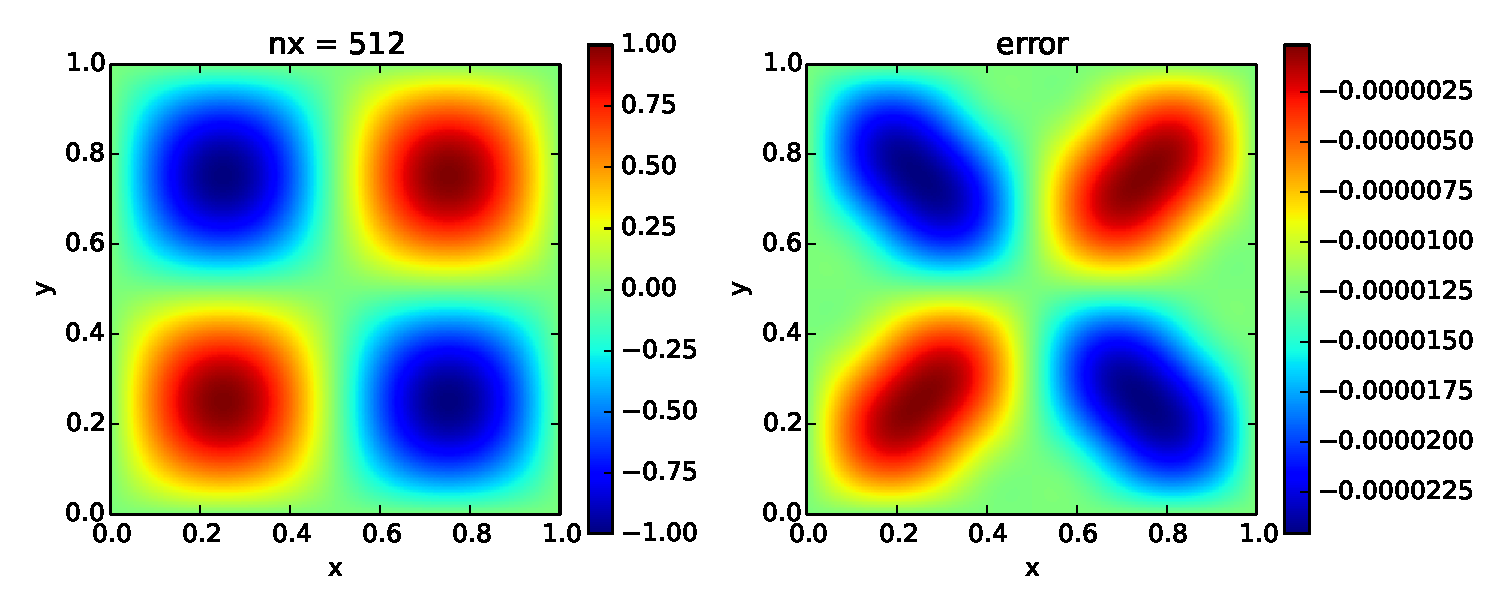
\includegraphics[width=\linewidth]{mg_vc_periodic_test}
\caption[Solution and error of a variable-coefficient Poisson problem]{\label{fig:mg_vc} Solution and error to the variable-coefficient 
Poisson problem defined in Eq.~\ref{eq:vc:lap}.  This test can be
run with \pyro\ {\tt multigrid/test\_mg\_vc\_periodic.py}.}
\end{figure}

\begin{figure}[t]
\centering
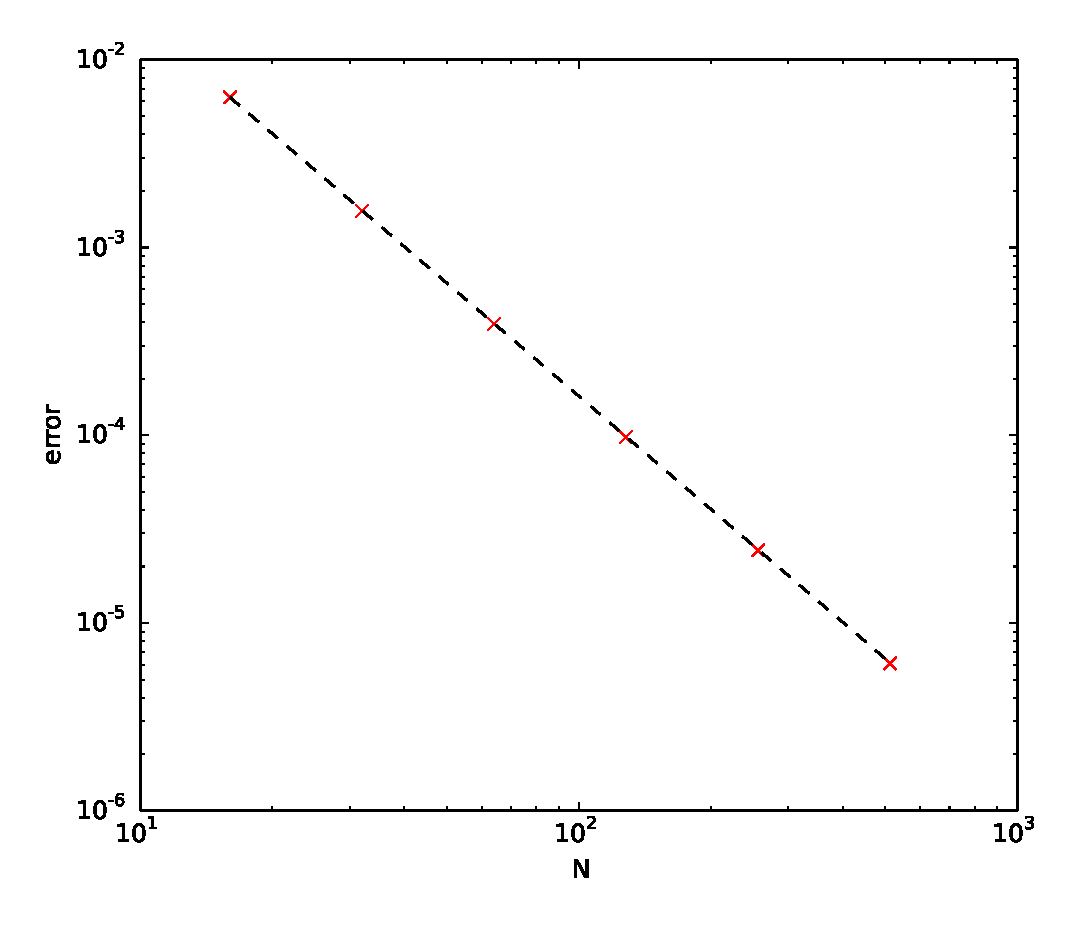
\includegraphics[width=0.8\linewidth]{mg_vc_periodic_converge}
\caption[Convergence of the variable-coefficient Poisson solver]{\label{fig:mg_vc_converge} Convergence of the variable-coefficient
multigrid solver for the test problem defined in Eq.~\ref{eq:vc:lap}.  This test can be
run with \pyro\ {\tt multigrid/test\_mg\_vc\_periodic.py}.}
\end{figure}

\subsubsection{Dirichlet}

We can run the same problem with Dirichlet boundary conditions on $\phi$,
and we are free to pick different boundary conditions for $\eta$, since
it represents a different physical quantity.  Since we only have homogeneous
Dirichlet or Neumann BCs implemented, we'll run with Neumann BCs on $\eta$.



\section{Atmospheric flows}
\label{sec:lm:atm} 

\subsection{Equation Set}

For atmospheric flows, we define a one-dimensional base state that is
in hydrostatic equilibrium.  In general, this base state can be
time-dependent, expanding in response to heating in the atmosphere
(see e.g. \cite{almgren:2000,ABRZ:II}.  Here we'll consider only a
time-independent state.

We'll follow the procedure defined in \cite{multilevel}: we define
$\rho_0$ as the lateral average of $\rho$:
\begin{equation}
{\rho_0}_j = \frac{1}{N_x} \sum_i \rho_{i,j}
\end{equation}
and then we define the base state pressure, $p_0$, by integrating the
equation of hydrostatic equilibrium, $dp_0/dy = \rho g$, as:
\begin{equation}
{p_0}_{j+1} = {p_0}_j + \frac{\Delta y}{2} ({\rho_0}_j + {\rho_0}_{j+1}) g
\end{equation}
with an initial condition of 
\begin{equation}
{p_0}_\mathrm{jlo} = \frac{1}{N_x} \sum_{i} p^\mathrm{initial}_{i,\mathrm{jlo}}
\end{equation}

The compressible momentum equation (written in terms of velocity is):
\begin{equation}
\rho \frac{\partial U}{\partial t} + \rho U \cdot \nabla U + \nabla p = \rho g
\end{equation}
Subtracting off the base state, and defining the perturbational
pressure (sometimes called the dynamic pressure) as $p^\prime = p -
p_0$, and perturbational density as $\rho' = \rho - \rho_0$, we have:
\begin{equation}
\rho \frac{\partial U}{\partial t} + \rho U \cdot \nabla U + \nabla p' = \rho' g
\end{equation}
or 
\begin{equation}
\frac{\partial U}{\partial t} + U \cdot \nabla U + \frac{1}{\rho} \nabla p^\prime = 
   \frac{\rho^\prime}{\rho} g
\end{equation}

Several authors \cite{KP:2012,VLBWZ:2013} explored the idea of energy
conservation in a low Mach number system and found that an additional term (which can
look like a buoyancy) is needed in the low Mach number formulation, yielding:
\begin{equation}
\frac{\partial U}{\partial t} + U \cdot \nabla U + 
   \frac{\beta_0}{\rho} \nabla \left (\frac{p^\prime}{\beta_0} \right ) = 
   \frac{\rho^\prime}{\rho} g
\end{equation}

Completing the system are the continuity equation,
\begin{equation}
\frac{\partial \rho}{\partial t} + \nabla \cdot (\rho U) = 0
\end{equation}
and the constraint,
\begin{equation}
\nabla \cdot (\beta_0 U) = 0
\end{equation}
with $\beta_0 = p_0^{1/\gamma}$.

  
\subsection{Solution Procedure}

\label{sec:lm:density}

The general solution procedure is for a single step is:
\begin{enumerate}
  \renewcommand{\labelenumi}{\Roman{enumi}.}
  
\item {\em Predict $U$ to the interfaces}

\item {\em Enforce the divergence constraint on the interface $U$'s (the
  MAC projection) to get $U^\mathrm{adv}$.}

  Decomposing the velocity field as
  \begin{equation}
    U^\star = U^d + \frac{\beta_0}{\rho} \nabla \phi
  \end{equation}
  as suggested from the form of the momentum equation, our Poisson
  equation can be defined by multiplying by $\beta_0$ and taking the
  divergence, and using $\nabla \cdot (\beta_0 U^d) = 0$, giving
  \begin{equation}
    \nabla \cdot \frac{\beta_0^2}{\rho} \nabla \phi =
    \nabla \cdot (\beta_0 U^\star)
  \end{equation}
  Note that when written like this, $\phi$ has units of
  $p^\prime/\beta_0$. \MarginPar{there is a $\Delta t$ here too}
  
  For the MAC projection, we have edge-centered velocities (in their
  respective coordinate direction).  We define an edge-centered $\beta_0$ as
  \begin{equation}
    {\beta_0}_{j+1/2} = \frac{1}{2} ( {\beta_0}_j + {\beta_0}_{j+1} )
  \end{equation}
  (note that, since $\beta_0$ is one-dimensional, we only average in
  the vertical direction).  The divergence term is then:
  \begin{equation}
    \left [ \nabla \cdot (\beta_0 U) \right ]_{i,j}^\mathrm{adv} =
          {\beta_0}_j \frac{u^\mathrm{adv}_{i+1/2,j} - 
            u^\mathrm{adv}_{i-1/2,j}}{\Delta x} +
          \frac{{\beta_0}_{j+1/2} v^\mathrm{adv}_{i,j+1/2} - 
            {\beta_0}_{j-1/2} v^\mathrm{adv}_{i,j-1/2} }{\Delta y}
  \end{equation}
  
  We define the coefficient, $\eta$, in the Poisson equation as:
  \begin{equation}
    \eta_{i,j} = \frac{{\beta_0}_j^2}{\rho_{i,j}}
  \end{equation}
  and bring it to edges simply through averaging.  Multigrid is
  used to solve for $\phi_{i,j}$.

  We then solve
  \begin{equation}
    (L_\eta\phi)_{i,j} =
    \left [ \nabla \cdot (\beta_0 U) \right ]_{i,j}^\mathrm{adv}
  \end{equation}
  Once we solve for $\phi$, we correct the velocity as:
  \begin{equation}
    U^\mathrm{new} = U^\star - \frac{\beta_0}{\rho} \nabla \phi
  \end{equation}
  Since the MAC velocities are edge-centered, our correction appears as:
  \begin{align}
    u^\mathrm{adv}_{i+1/2,j} &= u^\mathrm{adv}_{i+1/2,j} -
    \left (\frac{\beta_0}{\rho}\right )_{i+1/2,j}
    \frac{\phi_{i+1,j} - \phi_{i,j}}{\Delta x} \\
    %
    v^\mathrm{adv}_{i,j+1/2} &= v^\mathrm{adv}_{i,j+1/2} -
    \left (\frac{\beta_0}{\rho}\right )_{i,j+1/2}
    \frac{\phi_{i,j+1} - \phi_{i,j}}{\Delta y} 
  \end{align}
  
\item {\em Predict $\rho$ to the interfaces}

We need to solve the continuity equation.  We use the same techniques
that were used for advection.  Our equation is:
\begin{equation}
\rho_t + (\rho u)_x + (\rho v)_y = 0
\end{equation}
The $x$-interface left state would be:
\begin{align}
\rho_{i+1/2,j,L}^{n+1/2} &= \rho_{i,j}^n + 
   \frac{\Delta x}{2} \frac{\partial \rho}{\partial x} +
   \frac{\Delta t}{2} \frac{\partial \rho}{\partial t} + \ldots \nonumber \\
%
 &= \rho_{i,j}^n + 
    \frac{\Delta x}{2} \frac{\partial \rho}{\partial x} +
    \frac{\Delta t}{2} \left [ -(\rho u)_x -(\rho v)_y \right ]_{i,j} \nonumber\\
%
 &= \underbrace{\rho_{i,j}^n + 
   \frac{\Delta x}{2} \left ( 1 - \frac{\Delta t}{\Delta x} u_{i,j} \right )
        \frac{\partial \rho}{\partial x}}_{\hat{\rho}_{i+1/2,j,L}^{n+1/2}}
   - \frac{\Delta t}{2} \left [\rho u_x \right ]_{i,j} 
   - \frac{\Delta t}{2} \left [ (\rho v)_y \right ]_{i,j}
\end{align}
A similar construction would yield the right state at that interface, and the
$y$-interface states.

Since we already have the MAC-projected advected velocities at this
point, we can use them in the construction of the interface states and
the upwinding.  As before, we split this into a normal part (the
$\hat{\rho}$ term) and ``transverse'' part (which here includes the
non-advective part of the divergence).  We first construct the normal
parts as
\begin{equation}
\hat{\rho}_{i+1/2,j,L}^{n+1/2} = \rho_{i,j}^n + 
   \frac{1}{2} \left ( 1 - \frac{\Delta t}{\Delta x} u^\mathrm{adv}_{i+1/2,j} \right )
   \overline{\Delta \rho}^{(x)}_{i,j}
\end{equation}
and then solve the Riemann problem (upwinding) for these:
\begin{equation}
\hat{\rho}_{i+1/2,j}^{n+1/2} = 
   \mathcal{U}[u^\mathrm{adv}_{i+1/2,j}](\hat{\rho}_{i+1/2,j,L}^{n+1/2},
                                     \hat{\rho}_{i+1/2,j,R}^{n+1/2}) =
  \left \{
  \begin{array}{cl}
     \hat{\rho}_{i+1/2,j,L}^{n+1/2} & u^\mathrm{adv}_{i+1/2,j} > 0 \\
     \hat{\rho}_{i+1/2,j,R}^{n+1/2} & u^\mathrm{adv}_{i+1/2,j} < 0 
  \end{array} \right .
\end{equation}
The same procedure is done for the $y$-interfaces.

The full states are then constructed using these ``hat'' states.  For example,
\begin{align}
\rho_{i+1/2,j,L}^{n+1/2} = \hat{\rho}_{i+1/2,j,L}^{n+1/2} 
   &- \frac{\Delta t}{2} \rho_{i,j} 
     \frac{u^\mathrm{adv}_{i+1/2,j} - u^\mathrm{adv}_{i-1/2,j}}{\Delta x} \nonumber \\
   &- \frac{\Delta t}{2} 
        \frac{\hat{\rho}_{i,j+1/2}^{n+1/2} v^\mathrm{adv}_{i,j+1/2} -
              \hat{\rho}_{i,j-1/2}^{n+1/2} v^\mathrm{adv}_{i,j-1/2}}{\Delta y}
\end{align}
Once the new states on both the $x$- and $y$-interfaces are constructed, we
again upwind to find the final $\rho$ state on each interface:
\begin{equation}
\rho_{i+1/2,j}^{n+1/2} = 
   \mathcal{U}[u^\mathrm{adv}_{i+1/2,j}](\rho_{i+1/2,j,L}^{n+1/2},
                                     \rho_{i+1/2,j,R}^{n+1/2}) =
  \left \{
  \begin{array}{cl}
     \rho_{i+1/2,j,L}^{n+1/2} & u^\mathrm{adv}_{i+1/2,j} > 0 \\
     \rho_{i+1/2,j,R}^{n+1/2} & u^\mathrm{adv}_{i+1/2,j} < 0 
  \end{array} \right .
\end{equation}


  
\item {\em Do the conservative update of $\rho$}

  Once the interface states are found, we can conservatively-difference
the continuity equation:
\begin{align}
\rho^{n+1}_{i,j} = \rho^n_{i,j} 
   &- \frac{\Delta t}{\Delta x} 
      \left (\rho_{i+1/2,j}^{n+1/2} u^\mathrm{adv}_{i+1/2,j} -
             \rho_{i-1/2,j}^{n+1/2} u^\mathrm{adv}_{i-1/2,j} \right ) \nonumber \\
   &- \frac{\Delta t}{\Delta y}
      \left (\rho_{i,j+1/2}^{n+1/2} v^\mathrm{adv}_{i,j+1/2} -
             \rho_{i,j-1/2}^{n+1/2} v^\mathrm{adv}_{i,j-1/2} \right )
\end{align}


\item {\em Update $U^n$ to $U^{n+1,\star}$}
  
\item {\em Enforce the divergence constraint on $U^{n+1}$}

  For the final projection, we have cell-centered velocties.  We 
  define the divergence term as:
  \begin{equation}
    \left [ \nabla \cdot (\beta_0 U) \right ]_{i,j}^\star =
          {\beta_0}_j \frac{u^\star_{i+1,j} - 
            u^\star_{i-1,j}}{2\Delta x} +
          \frac{{\beta_0}_{j+1} v^\star_{i,j+1} - 
            {\beta_0}_{j-1} v^\star_{i,j-1} }{2\Delta y}
  \end{equation}

  
\end{enumerate}


\subsection{Timestep constraint}

In addition to the advective timestep constraint, an additional constraint
is needed if the velocity field is initialially zero.  In \cite{ABNZ:III},
a constraint based on the buoyancy forcing is used.  First, we compute
the maxiumum buoyancy acceleration,
\begin{equation}
a_\mathrm{max} = \max \left \{ \left |\frac{\rho'g}{\rho} \right | \right \}
\end{equation}
and then 
\begin{equation}
\Delta t_\mathrm{force} = \left ( \frac{2 \Delta x}{a_\mathrm{max}} \right )^{1/2} 
\end{equation}
This is based simply on $\Delta x = (1/2) a t^2$---the
time it takes for the buoyant force to accelerate a fluid element
across a zone width.


\subsection{Bootstrapping}

First we need to make sure that the initial velocity field satisfies our constraint

Next we need to find $\nabla {p^\prime}^{n-1/2}$ for the first step.



\section{Combustion}


Taking $p = p_0 + p^\prime$, with $p_0 = \mathrm{constant}$, the system 
becomes:
\begin{align}
\frac{\partial \rho}{\partial t} + \nabla \cdot (\rho U) &= 0 \\
\frac{\partial \rho U}{\partial t} + \nabla \cdot (\rho U U) + \nabla p^\prime &= 0 \\
\nabla \cdot U &= S
\end{align}

\subsection{Species}


\subsection{Constraint}

Our constraint equation is $\nabla \cdot U = S$.  Decomposing the
velocity field as
\begin{equation}
U^\star = U^d + \frac{1}{\rho} \nabla \phi
\end{equation}
our Poisson equation can be defined by taking the divergence, and
using $\nabla \cdot U^d = S$, giving
\begin{equation}
\nabla \cdot \frac{1}{\rho} \nabla \phi = \nabla \cdot U^\star - S
\end{equation}


\subsection{Solution Procedure}

The general solution procedure is for a single step is:
\begin{itemize}

  \item React for $\Delta t/2$

  \item Do the hydrodynamcis for $\Delta t$

    \begin{itemize}
    \item Predict $U$ to the interfaces 
    \item Enforce the divergence constraint on the interface $U$'s (the
      MAC projection) to get $U^\mathrm{adv}$.
    \item Predict $\rho$ to the interfaces
    \item Do the conservative update of $\rho$
    \item Update $U^n$ to $U^{n+1}$
    \item Enforce the divergence constraint on $U^{n+1}$
    \end{itemize}

  \item React for $\Delta t/2$

\end{itemize}
